\documentclass{article}

% english 
\usepackage[utf8]{inputenc}

% reduced margins
\usepackage{fullpage}

% maths
\usepackage{amsmath}
\usepackage{amssymb}

% algorithms
\usepackage{algorithm}
\usepackage[noend]{algpseudocode}

% url
\usepackage{hyperref}

% graphics
\usepackage{graphicx}

% float
% especially to force text not to skip images
\usepackage{float}

% metadata
\title{Stochastic Dual Coordinate Descent}
\author{Guillaume Desforges \& Michaël Karpe \& Matthieu Roux}
\date{June 14th 2018}

% custom commands
\newcommand{\abs}[1]{\left|#1\right|}
\newcommand{\norm}[1]{\left\|#1 \right\|}

% custom display
\setlength{\parskip}{0.3em}
\setlength{\parindent}{0em}

\begin{document}

\maketitle

%=================================================================================================
\section*{Introduction}

% Context
\hspace{2em}
In machine learning, the process of fitting a model to the data requires to solve an optimization problem.
The difficulty resides in the fact that this optimization quickly becomes very complex when dealing with real problems.
The Stochastic Gradient Descent (SGD) is a very popular algorithm to solve those problems because it has good convergence guaranties.
Yet, the SGD does not have a good stopping criteria, and its solutions are often not accurate enough.

% General problem studied, general methodology
\hspace{2em}
The Stochastic Dual Coordinate Ascent (SDCA) tries to solves the optimization problem by solving its dual problem.
Instead of optimizing the weights, we optimize a dual variable from which we can compute the weights and thus solve the former.
This method can give good results for specific problems : for instance, solving the dual problem of the SVM has proven to be effective and to give interesting results, with a linear convergence in some cases.

% Focus and goal of the work presented
\hspace{2em}
In this report, we compile the key theoretical points necessary to have a global understanding of the SDCA.

% Structure of the report
\hspace{2em}
First we introduce the SDCA and its principles.
We then present the machine learning problem our report focuses on.
Then we study computational performances of the method by trying to apply SDCA on concret problems.
Finally we conclude on SDCA strengths and weaknesses.

\paragraph{Note} \textit{We especially added experimentations since the presentation of our poster.}


%=================================================================================================
\section{Purpose of the report: a new SGD-like method}
% 3 pages
% (a) [DONE] ...... specific problem studied
% (c) [DONE] ...... model, main idea
% (d) [IRRELEVANT]  specific methodology
% (e) [DONE] ...... algorithms

\subsection{Difference between SGD and SDCA}

%A REFORMULER : COPIER / COLLER DE L'ARTICLE !
%Surtout que eps_P sub optimal est défini plus loin...

\hspace{2em}
A simple approach for solving Support Vector Machine learning is Stochastic gradient Descent (SGD).
SGD finds an $\epsilon_P$-sub-optimal solution in time $O(1/(\lambda \epsilon_P))$.
This runtime does not depend on $n$ and therefore is favorable when $n$ is very large.
However, the SGD approach has several disadvantages:

\begin{enumerate}
    \item it does not have a clear stopping criterion
    \item it tends to be too aggressive at the beginning of the optimization process, especially when $\lambda$ is very small
    \item while SGD reaches a moderate accuracy quite fast, its convergence becomes rather slow when we are interested in more accurate solutions
\end{enumerate}

\hspace{2em}
Therefore, an alternative approach is Dual Coordinate Ascent (DCA), which solves the dual problem instead of the primal problem.

\subsection{General SDCA procedure}

Let $x_1, \dots, x_n \in \mathbb{R}^d$, $\phi_1, \dots, \phi_n$ scalar convex functions, $\lambda > 0$ regularization parameter.

Let us focus on the following optimization problem:
\begin{equation}
    \min_{w \in \mathbb{R}^d} P(w) = \left[ \dfrac{1}{n} \sum_{i=1}^n \phi_i(w^\top x_i) + \dfrac{\lambda}{2}\norm{w}^2 \right]
    \label{primal}
\end{equation}
with solution $w^{*} = \arg \min_{w \in \mathbb{R}^d} P(w)$.

We say that a solution $w$ is $\epsilon_P$-sub-optimal if $P(w) - P(w^{*}) \leq \epsilon_P$.

We analyze here the required runtime to find an $\epsilon_P$-sub-optimal solution using SDCA.

Let $\phi_i^{*} : \mathbb{R} \rightarrow \mathbb{R}$ be the convex conjugate of $\phi_i$ : $\phi_i^{*}(u) = \max_z (zu-\phi_i(z))$.
The dual problem of \eqref{primal} is defined as follows:
\begin{equation}
    \max_{\alpha \in \mathbb{R}^n} D(\alpha) = \left[ \dfrac{1}{n} \sum_{i=1}^n -\phi_i^{*}(-\alpha_i) - \dfrac{\lambda}{2}\norm{\dfrac{1}{\lambda n}\sum_{i=1}^n \alpha_ix_i}^2 \right]
    \label{dual}
\end{equation}
with solution $\alpha^{*} = \arg \max_{a \in \mathbb{R}^n} D(\alpha)$.

We define $w(\alpha) = \frac{1}{\lambda n} \sum_{i=1}^n \alpha_ix_i$.
Thanks to classic optimization results, we then have :

\begin{equation}
	w(\alpha^{*}) = w^{*}
\end{equation}
\begin{equation}
	P(w^{*}) = D(\alpha^{*})
\end{equation}
\begin{equation}
	\forall (w,\alpha), P(w) = D(\alpha)
\end{equation}

We define the duality gap as $P(w(\alpha)) - P(w^{*})$.

The SDCA algorithm is described further.
$T_0$ can be chosen between $1$ to $T$, and is generally chosen equal to $T/2$.
However, in pratice, these parameters are not required as the duality gap is used to terminate the algorithm.

\subsection{Focus on the logistic regression}

In order to fully grasp the method behind the first paper, let's take an example with the logistic regression.
We will consider logistic regression only for binary classification.

We use the following usual notations : $X \in \mathbf{X} = \mathbb{R}^p$ the random variable for the description space, and $Y \in \mathbf{Y} = \{-1,1\}$ the random variable for the label.

We recall that the model is the following :
\begin{equation}
	\frac{\mathbb{P}(y=1 | X=x)}{\mathbb{P}(y=-1 |X=x)} = w^T x, \quad w \in \mathbb{R}^p
\end{equation}

We want to find $w$ such that it maximizes the likelihood, or log-likelihood, with a term of regularization:
\begin{equation}
	\min_w C \sum_i \log\left(1 + e^{-y_iw^Tx_i}\right)  + \frac{1}{2} w^Tw
\end{equation}

In order to get the dual problem, we rewrite it with an artificial constraint $z_i = e^{-y_iw^Tx_i}$, and we have the following lagrangian :
\begin{equation}
	\mathcal{L}(w, z, \alpha) = \sum_i (C \log\left(1+z_i\right) + \alpha_i z_i) - \sum_i \alpha_i e^{-y_iw^Tx_i} + \frac{1}{2}w^Tw 
\end{equation}

We will note $w^* = \sum_i \alpha_i y_i x_i$ and $z^*$ the variables solution of the optimization problem
\begin{equation}
	\min_{w, z} \mathcal{L}(w, z, \alpha) = \mathcal{L}(w^*, z^*, \alpha) = \psi(\alpha) 
\end{equation}

In fact, it leads to the following dual problem :
\begin{equation}
	\begin{aligned}
		& \max_{\alpha} & &\sum_{i \in I} (-\alpha_i \log(\alpha_i) - (C-\alpha_i) \log(C - \alpha_i)) - \frac{1}{2} \alpha^TQ\alpha\\
		& s.t.          & &I = \{i,\ 0 < \alpha_i < C \}\\
		&               & &0 \leq \alpha_i \leq C
	\end{aligned}
\end{equation}

Now we got the dual problem, we need to solve a maximization problem.
To do so, we will use in this paper the coordinate ascent method, which consist in optimizing the objective function coordinate by coordinate (or with groups of coordinates).
The SDCA algorithm is described in the next subsection.

\subsection{SDCA algorithm}

\begin{algorithm}[H]
    \caption{Procedure SCDA}
    \begin{algorithmic}
        \Procedure{SCDA}{$\alpha^{(0)},\phi, T_0, T$}
        \State $w^{(0)} \gets w(\alpha^{(0)})$
        \For{$t = 1, \dots, T$} %FOR
        \State Randomly pick $i$
        \State $\Delta \alpha_i \gets \arg \max -\phi^{*}_i(-(\alpha_i^{(t-1)}+\Delta \alpha_i))-\frac{\lambda n}{2}\norm{w^{(t-1)}+(\lambda n)^{-1}\Delta \alpha_i x_i}^2$ \qquad \qquad \qquad \qquad \qquad (*)
        \State $\alpha^{(t)} \gets \alpha^{(t-1)} + \Delta \alpha_i e_i$
        \State $w^{(t)} \gets w^{(t-1)} + (\lambda n)^{-1} \Delta \alpha_i x_i$
        \EndFor
        \If{Averaging option}
        \State \textbf{return} $\overline{w} = \frac{1}{T-T_0} \sum_{i = T_0+1}^T w^{(t-1)}$
        \EndIf
        \If{Random option}
        \State \textbf{return} $\overline{w} = w^{(t)}$ for a random $t \in [|T_0+1, T|]$
        \EndIf
        \EndProcedure
    \end{algorithmic}
\end{algorithm}


\subsection{Computation of closed forms}

\hspace{2em}
In the studied articles, SDCA is computed either for $L$-Lipschitz loss functions or for $(1/\gamma)$-smooth loss functions.
We recall that a function $\phi_i : \mathbb{R} \rightarrow \mathbb{R}$ is $L$-Lipschitz if $\forall a,b \in \mathbb{R}$, $\abs{\phi_i(a)-\phi_i(b)} \leq L \abs{a-b}$, and that a function $\phi_i : \mathbb{R} \rightarrow \mathbb{R}$ is $(1/\gamma)$-smooth if it is differentiable and its derivative is (1/$\gamma)$-Lipschitz.
Moreover, if $\phi_i$ is $(1/\gamma)$-smooth, then $\phi_i^{*}$ is $\gamma$-strongly convex.
The different loss functions used are described in the table below.
For experimentation, we mainly focused on log loss and square loss.

\hspace{2em}
Some loss functions used in the report are described in the table in appendix \ref{appendix-losses}.

\subsection{Algorithm termination}

For the sake of simplicity, the studied articles consider the following assumptions: $\forall i, \norm{x_i} \leq 1$, $\forall (i,a), \phi_i(a) \geq 0$ and $\forall i, \phi_i(0) \leq 1$.
Under these assumptions, we have the following theorem:

\paragraph{Theorem} Consider Procedure SDCA with $\alpha^{(0)} = 0$.
Assume that $\forall i, \phi_i$ is $L$-Lipschitz (resp. $(1/\gamma)$-smooth).
To obtain an expected duality gap of $\mathbb{E}[P(\overline{w})-D(\overline{\alpha})] \leq \epsilon_P$, it suffices to have a total number of iterations of
$$T \geq n + \max\left(0, \left\lceil n \log \left(\dfrac{\lambda n}{2 L^2} \right) \right\rceil \right) + \dfrac{20 L^2}{\lambda \epsilon_P} \quad \left( \text{resp. } T > \left(n + \dfrac{1}{\lambda \gamma} \right) \log \left[ \dfrac{1}{(T-T_0)\epsilon_P} \left(n + \dfrac{1}{\lambda \gamma} \right) \right] \right)$$ 


%=================================================================================================
\section{Experiments}
% 2 pages
% (a) Description of the dataset(s) considered / general problem associated with the data \\
% (b) Description of the protocol of the experiments (setting of the hyperparameters/cross-validation procedure/evaluation methodology) \\
% (c) Factual description of the type of results reported (explanation pertaining to the Figures, tables, etc) \\
% (d) Interpretation and discussion of the results (comparison with the baselines, advantages of each algorithm, etc) \\

\subsection{Implementation}

The experiments in this report were done with our own implementation, available on GitHub :

\url{ https://github.com/GuillaumeDesforges/enpc-malap-project-sdca }

We implemented :

\begin{itemize}
	\item \texttt{Estimator} objects that can fit, predict and score themselves : logistic loss and square loss
	\item \texttt{Optimizer} objects used for fitting : SGD and SDCA
	\item projections : polynomial and gaussian
	\item some data utilities
\end{itemize}

\subsection{Description of the chosen datasets}

We used our implementation on :

\begin{itemize}
	\item Two gaussians to check that our implementation works
	\item \textit{Arrhythmia} : \url{https://archive.ics.uci.edu/ml/datasets/Arrhythmia}
	\item \textit{Adults} : \url{https://archive.ics.uci.edu/ml/datasets/adult}
\end{itemize}

While the Arrhythmia dataset has 452 instances, which is quite low, it has 279 features, which is quite high.
On the other hand, the Adult dataset has 48842 instances but only 14 features.

The Arrhythmia dataset will help us check the properties of SDCA when there are many features.
The Adult dataset will help us compare the SGD and SDCA when there are many instances.

\subsection{Use of closed forms and numerical issues}

In this report, we used the closed form presented above.
The closed form for the logistic regression gave us numerous numerical issues.

% TODO développer

% TODO supprimer ces commentaires
% C'EST l'INVERSE !!! @MichaelKarpe
% le papier sur la forme non close passe son temps à vouloir régler les problèmes numériques
% After having fixed or bypassed numeric issues thanks to the use of closed forms, we can discuss the choice of the different parameters.

A solution that is proposed by another study is to optimize a subproblem with a modified Newton algorithm for each iteration, and thus avoid catastrophic cancelations.

\subsection{Choice of algorithm termination option}

Because of the stochastic behavior of the algorithm, the output is very sensitive to the iteration at which it stops.
Indeed, coefficients vary suddenly, and the convergence is not really monotonous : at some point, it is uncertain whether the loss improves or not.

There are essentially two ways of taking this into account.
The first method is to stop at a random step, which actually yields good results.
The second method consists in averaging the last $\alpha^{(t)}$ obtained by the algorithm, making sure that the local variations of $\alpha$ are corrected.

% TODO parler de la terminaison par le duality gap !
% Il aurait fallu regarder si les conditions sur le nb d'itérations sont bien vérifiées ou pas

% Transition : 
Considering this analysis, and as we did not achieve to check the theorem in Section 2.6., we decided to choose the average output option and to set $T_0 = T/2$, as suggested in the studied articles.

\subsection{Choice of hyperparameters}

The SGD has two hyperparameters \texttt{c} and \texttt{eps} while the SDCA has only one hyperparameter \texttt{c}.

In order to compare the algorithm, we chose to select the best hyperparameters for each optimizer and for each data set.

On every data set, for each hyperparameter, We computed the accuracy after a given number of epochs for a range of values, and plotted them.

\begin{figure}[H]
	\centering
	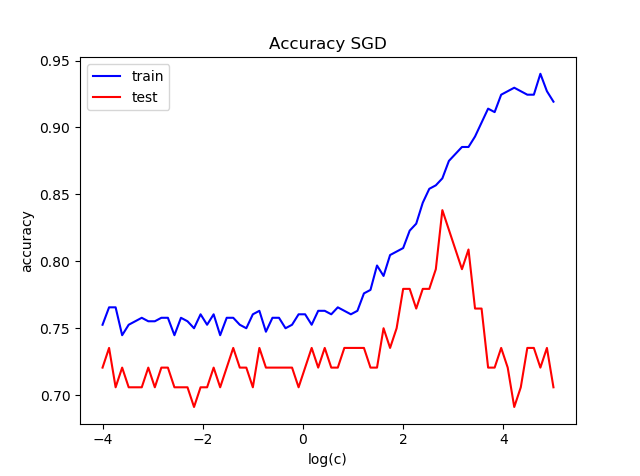
\includegraphics[height=6cm]{figs/hyperparams/SGD_c.png}
	\caption{Selection of the hyperparameter \texttt{c} for the SGD for the dataset Arrhythmia}
\end{figure}

\begin{figure}[H]
	\centering
	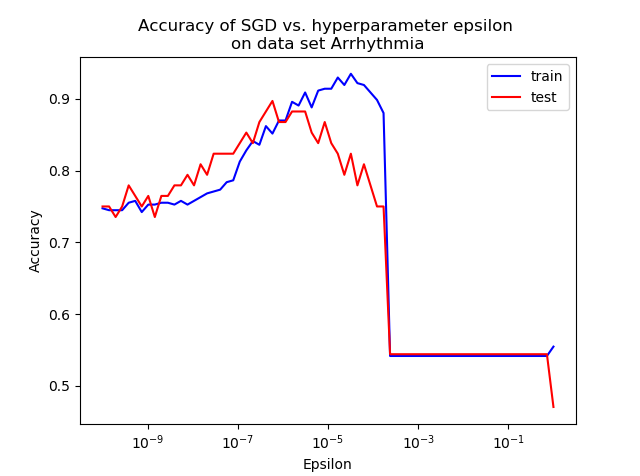
\includegraphics[height=6cm]{figs/hyperparams/SGD_eps.png}
	\caption{Selection of the hyperparameter \texttt{eps} for the SGD for the dataset Arrhythmia}
\end{figure}

\begin{figure}[H]
	\centering
	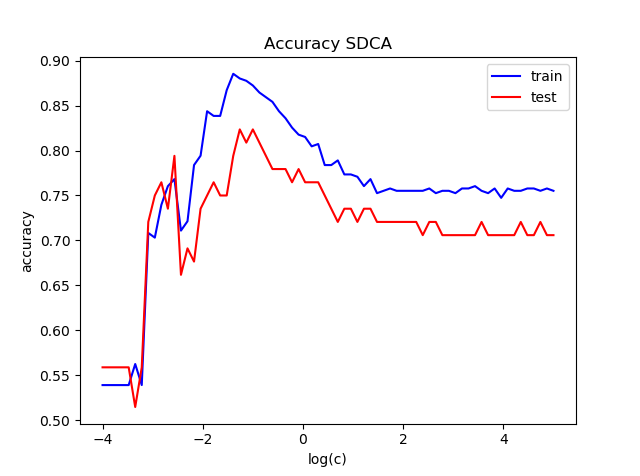
\includegraphics[height=6cm]{figs/hyperparams/SDCA_c.png}
	\caption{Selection of the hyperparameter \texttt{c} for the SDCA for the dataset Arrhythmia}
\end{figure}

We selected the hyper parameters values :

\begin{table}[H]
	\centering
	\begin{tabular}{|r|c|c|c|}
		\hline
		Data set & SGD \texttt{c} & SGD \texttt{eps} & SDCA \texttt{c}\\
		\hline
		Arrhythmia & 1 & 1 & 1\\
		Adults & 1 & 1 & 1\\
		\hline
	\end{tabular}
	\caption{Hyper parameter values used}
\end{table}

\subsection{Comparison between SGD and SDCA on used datasets}

Lorem ipsum.


%=================================================================================================
\section*{Conclusion}
% 1/2 page
% (a) summary \\
% (b) main conclusions and take home messages \\
% (c) Remaining questions/ future directions (only if relevant) \\


%=================================================================================================
\section*{References}

% TODO references

\newpage
\appendix
%=================================================================================================
\section{Losses used}
\label{appendix-losses}

\begin{center}
	\begin{table}[H]
		\centering

		\begin{tabular}{|c|}
			\hline

			\textbf{Squared loss:}\\[1.3em]
			$\phi_i(a) = (a-y_i)^2$\\[1.3em]
			$\phi_i^{*}(-a) = -ay_i+a^2/4$\\[1.3em]
			$\Delta \alpha_i = \dfrac{y_i-x_i^\top w^{(t-1)}-0.5\alpha_i^{(t-1)}}{0.5+\norm{x_i}^2/(\lambda n))}$\\[1.3em]

			\hline

			\textbf{Absolute deviation loss:}\\[1.3em]
			$\phi_i(a) = \abs{a-y_i}$ \\[1.3em]
			$\phi_i^{*}(-a) = -ay_i$, $a \in [-1,1]$\\[1.3em]
			$\Delta \alpha_i = \max \left( 1, \min \left( 1, \dfrac{y_i-x_i^\top w^{(t-1)}}{\norm{x_i}^2/(\lambda n)} + \alpha_i^{(t-1)} \right) \right) - \alpha_i^{(t-1)}$\\[1.3em]
			
			\hline

			\textbf{Log loss:}\\[1.3em]
			$\phi_i(a) = \log(1+\exp(-y_ia))$\\[1.3em]
			$\phi_i^{*}(-a) = -ay_i\log(ay_i) + (1-ay_i)\log(1-ay_i)$\\[1.3em]
			$\Delta \alpha_i = \dfrac{(1+\exp(x_i^\top w^{(t-1)}y_i))^{-1}y_i-\alpha_i^{(t-1)}}{\max(1,0.25+\norm{x_i}^2/(\lambda n))}$\\[1.3em]

			\hline

			\textbf{($\gamma$-smoothed) Hinge loss:}\\[1.3em]
			$\phi_i(a) = \max\{0,1-y_ia\}$\\[0.3em]
			$\phi_i^{*}(-a) = -ay_i + \gamma a^2/2$, $ay_i \in [0,1]$\\[1.3em]
			$\Delta \alpha_i = y_i \max \left( 0, \min \left( 1, \dfrac{1-x_i^\top w^{(t-1)} y_i-\gamma \alpha_i^{(t-1)}y_i}{\norm{x_i}^2/(\lambda n)+\gamma} + \alpha_i^{(t-1)} y_i \right) \right) - \alpha_i^{(t-1)}$\\[1.3em]

			\hline
		\end{tabular}

		\caption{Used loss functions, convex conjugates and closed form of solutions of problem (*).}
		\label{dataset}
	\end{table}
\end{center}

$\Delta \alpha_i$ is the notation we use to represent the increment to add to $\alpha_i$ (one coordinate, at a given iteration) to maximize the objective function with respect to that coordinate.


\end{document}

